\documentclass[11pt,a4paper]{article}
\usepackage[T1]{fontenc}
\usepackage[margin=2.3cm]{geometry}
\usepackage{amsmath,amssymb}
\usepackage{graphicx}
\usepackage[dvipsnames]{xcolor}
\usepackage{enumitem}
\usepackage[colorlinks=true,linkcolor=blue,urlcolor=blue]{hyperref}
\setlength{\parskip}{0.6em}
\setlength{\parindent}{0pt}
\begin{document}

\begin{center}{\LARGE\bfseries opendaylight}\\[0.4em]{\large Plan windows for natural daylight using the sun path, in three sessions.}\\[0.2em]\small PAN IIT OSS explainer \textbullet{} higher secondary to diploma / undergraduate (levels 4-5)\end{center}

\section*{Why this exists}
Window size and the sun path decide how much natural light a room gets and how much energy it needs. This explainer follows the idea from the sun's position in the sky to the shading of a window and a year-long simulation of a room, using only school trigonometry and an energy balance.

\section*{The end goal}
Plan windows for natural daylight using the sun path: know where the sun will be, choose the orientation, size and overhang of a window, and check with numbers that the room gets enough daylight for the least electricity. The same ideas apply to houses, classrooms, offices and solar panels.

\textit{This is a simplified educational model. It is not a validated design tool and must not be used for real structures, electrical installations, vehicles, industrial processes or medical decisions.}

\section*{How the three sessions build up}
\begin{enumerate}[nosep]
\item \textbf{Session 1: Where is the sun? Sun path, shadows and day length} (Level 1, conceptual interactive model, 60 min).
\item \textbf{Session 2: Sunlight on a window, the overhang and solar heat gain} (Level 2, mathematical engineering model, 75 min).
\item \textbf{Session 3: Simulate a year of daylight and heat, then plan the window} (Level 3, simulation and validation, 90 min).
\end{enumerate}

\section{Session 1: Where is the sun? Sun path, shadows and day length}

\subsection*{A. Real-world problem}
An architect in Delhi wants winter sun in a living room and a cool bedroom in May. A builder in Chennai wonders why the sun shines into a north window in June. Before anyone can size or shade a window they must know where the sun is: how high, in which direction, and for how long each day. How do we compute that from nothing more than the latitude, the date and the hour? (General education only: this is a simplified model, not a building design method.)

\subsection*{B. Concept and theory}
The Earth spins about an axis tilted 23.45 degrees from the plane of its orbit. Through the year the latitude where the noon sun is straight overhead moves between 23.45 N (about 21 June) and 23.45 S (about 21 December); that latitude is the \textbf{declination} delta. At \textbf{solar noon} the sun is in the north-south plane and the angle between the vertical and the sun is the difference phi - delta, so the noon altitude is 90 - |phi - delta|. The sun appears to turn 15 degrees per hour around the Earth's axis; the \textbf{hour angle} H = 15 (hour - 12) measures this. Projecting the sun direction onto east, north and up gives the \textbf{altitude} (angle above the horizon) and the \textbf{azimuth} (compass bearing, measured clockwise from north). A vertical pole of height h casts a shadow h / tan(altitude). Setting the altitude to zero gives the sunrise hour angle and so the day length. Times in this repo are \textbf{solar time}: 12:00 is when the sun crosses the meridian, which differs from clock time by up to about half an hour in India.

\begin{itemize}[nosep]
\item n: day of the year (1 = 1 January) (no unit)
\item delta: solar declination (degrees)
\item phi: latitude (north positive) (degrees)
\item H: hour angle, 15 x (solar hour - 12) (degrees)
\item alpha: sun altitude above the horizon (degrees)
\item A: sun azimuth, clockwise from north (S = 180) (degrees)
\item h, L: pole height, shadow length (m)
\end{itemize}

\begin{equation*}
\delta = 23.45^\circ \sin\!\left(\frac{360^\circ\,(284+n)}{365}\right)
\end{equation*}

\begin{equation*}
\alpha_{\mathrm{noon}} = 90^\circ - |\varphi - \delta|
\end{equation*}

\begin{equation*}
\sin\alpha = \sin\delta\sin\varphi + \cos\delta\cos\varphi\cos H,\qquad H = 15^\circ\,(t - 12)
\end{equation*}

\begin{equation*}
A = \operatorname{atan2}\big(-\cos\delta\sin H,\ \sin\delta\cos\varphi - \cos\delta\sin\varphi\cos H\big)
\end{equation*}

\begin{equation*}
L = \frac{h}{\tan\alpha},\qquad \cos H_0 = -\tan\varphi\tan\delta,\qquad \text{day length} = \frac{2H_0}{15^\circ}\ \text{h}
\end{equation*}

\begin{center}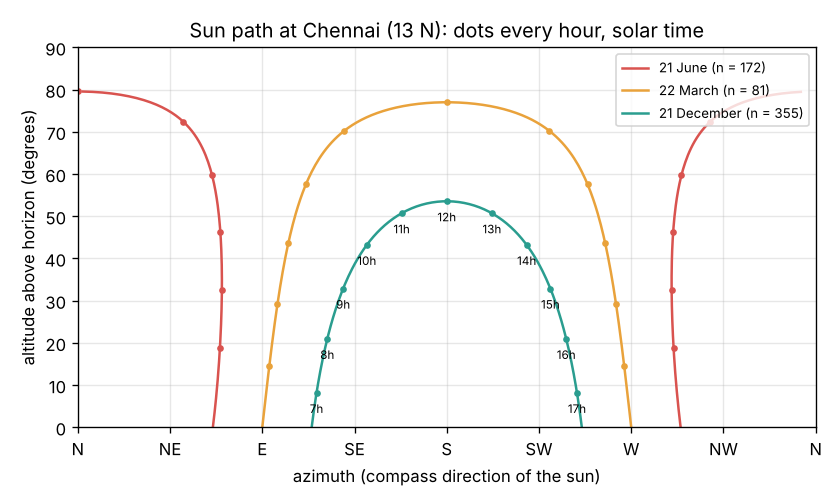
\includegraphics[width=0.85\linewidth]{figures/s01_sun_paths.png}\\\small Sun path at Chennai on 21 June, 22 March and 21 December, with hourly dots.\end{center}

\subsection*{E. Worked example}
In Delhi (latitude 28.6 N) on 21 December (n = 355), find the declination, the noon sun altitude, the noon shadow of a 2 m pole and the day length. Then find where the sun is at 9:00 solar time in Chennai (13 N) at the equinox.
\begin{enumerate}[nosep]
\item Declination: 360 x (284 + 355) / 365 = 630.25 degrees, sin(630.25) = -1.000, so delta = -23.45 degrees.
\item Noon altitude = 90 - |28.6 - (-23.45)| = 90 - 52.05 = 37.95 degrees. Since phi > delta the sun is due south.
\item Shadow = 2 / tan(37.95) = 2 / 0.780 = 2.56 m, pointing due north.
\item Day length: cos H0 = -tan(28.6) tan(-23.45) = 0.545 x 0.434 = 0.237, so H0 = 76.3 degrees and the day lasts 2 x 76.3 / 15 = 10.18 h.
\item Chennai, equinox, 9:00: H = -45, delta = 0, so sin(alpha) = cos(13) cos(45) = 0.689, alpha = 43.55 degrees. East part = sin(45) = 0.707, north part = -sin(13) cos(45) = -0.159, so the azimuth is atan2(0.707, -0.159) = 102.7 degrees (just south of east).
\end{enumerate}
\textbf{Answer.} delta = -23.45 degrees, noon altitude 37.95 degrees, shadow 2.56 m, day 10.18 h; at 9:00 in Chennai the sun is 43.55 degrees up at azimuth 102.7 degrees.

\subsection*{F. Questions}
\begin{enumerate}[nosep]
\item \textbf{Conceptual.} Why is the noon sun lower in winter than in summer in Delhi, and why can the noon sun be to the north in Chennai but never in Delhi?
\item \textbf{Numerical.} In Chennai on 21 June (delta = +23.45), find the noon sun altitude, the length and direction of the noon shadow of a 1 m pole, and the day length.
\item \textbf{Graph and simulation interpretation.} On the noon-shadow graph, how many times does the Chennai curve cross zero, and roughly on which days? Why does the Delhi curve never cross zero, and on which day is Delhi's noon shadow longest?
\item \textbf{Design and optimisation challenge.} Design: a courtyard house in Delhi has a 2.4 m high south wall of the next building 3 m away from your south window. Will the window get noon sun on 21 December? What is the shortest distance that keeps the whole window (sill at ground level) in noon sun on that day? Is the courtyard in shade at noon on 21 June?
\end{enumerate}

\section{Session 2: Sunlight on a window, the overhang and solar heat gain}

\subsection*{A. Real-world problem}
A west-facing bedroom in Chennai is hot every afternoon even with the curtains drawn, while a south-facing living room in Delhi gets pleasant winter sun under its chajja (concrete overhang) and stays shaded in summer. How much sunlight falls on a window that faces a given direction, how deep should the overhang be, and how many watts of heat does the sun push through the glass? (Simplified clear-sky model; not a building design method.)

\subsection*{B. Concept and theory}
A vertical wall faces the compass direction psi of its outward normal (south = 180). The \textbf{wall-solar azimuth} gamma = A - psi is how far round the sun is from straight in front. The \textbf{angle of incidence} theta between the sun's rays and the wall normal satisfies cos(theta) = cos(alpha) cos(gamma); if this is negative the sun is behind the wall. For shading we cut the wall in section: in that plane the sun ray makes the \textbf{vertical shadow angle} (VSA, or profile angle) with tan(VSA) = tan(alpha) / cos(gamma). An overhang of depth P a gap G above a window of height H throws its shadow P tan(VSA) down the wall, so the shaded height is clamp(P tan(VSA) - G, 0, H), and the whole window is shaded once P >= (G + H) / tan(VSA). A high VSA (summer noon on a south wall) is easy to cut off with a short overhang; a low VSA (morning sun on an east wall, afternoon sun on a west wall) needs an impossibly deep one. The strength of sunlight falls when it crosses more air: with air mass AM = 1 / sin(alpha), the Meinel clear-sky model gives the \textbf{direct normal irradiance} DNI = 1353 x 0.7\textasciicircum{}(AM\textasciicircum{}0.678) W/m2. A vertical wall also sees half of the sky's diffuse light, taken here as 0.05 DNI. The \textbf{solar heat gain coefficient} SHGC (0.6 for clear double glazing, roughly 0.8 for single clear glass) is the share of the sunlight hitting the glass that ends up as heat inside.

\begin{itemize}[nosep]
\item psi: direction the wall faces (N 0, E 90, S 180, W 270) (degrees)
\item gamma: wall-solar azimuth A - psi (degrees)
\item theta: angle of incidence on the wall (degrees)
\item VSA: vertical shadow angle in the wall section (degrees)
\item P, G, H, b: overhang depth, gap above window, window height, width (m)
\item DNI: direct normal irradiance (clear sky) (W/m2)
\item SHGC: solar heat gain coefficient of the glass (no unit)
\item Q: solar heat gain through the window (W)
\end{itemize}

\begin{equation*}
\cos\theta = \cos\alpha\,\cos\gamma,\qquad \gamma = A - \psi
\end{equation*}

\begin{equation*}
\tan(\mathrm{VSA}) = \frac{\tan\alpha}{\cos\gamma}
\end{equation*}

\begin{equation*}
\text{shaded height} = \min\!\big(\max(P\tan(\mathrm{VSA}) - G,\,0),\,H\big),\qquad P_{\mathrm{full}} = \frac{G + H}{\tan(\mathrm{VSA})}
\end{equation*}

\begin{equation*}
\mathrm{DNI} = 1353\times 0.7^{\,(1/\sin\alpha)^{0.678}}\ \mathrm{W/m^2}
\end{equation*}

\begin{equation*}
Q = \mathrm{SHGC}\; b\,H \left[\mathrm{DNI}\cos\theta\;f_{\mathrm{lit}} + 0.05\,\mathrm{DNI}\right]
\end{equation*}

\begin{center}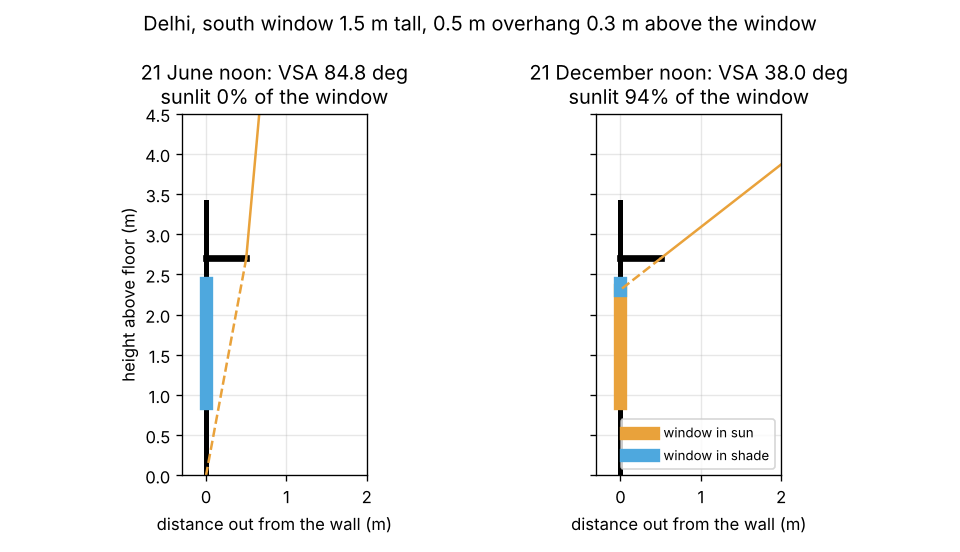
\includegraphics[width=0.85\linewidth]{figures/s02_overhang_section.png}\\\small A 0.5 m overhang in section: full shade at June noon, 94 percent sun at December noon (Delhi).\end{center}

\subsection*{E. Worked example}
A south window in Delhi (28.6 N) is 2 m wide and 1.5 m tall, with a 0.5 m overhang 0.3 m above it; SHGC = 0.6. Find the sunlit share and the solar heat gain at noon on 21 December, and check that the same overhang shades the window at noon on 21 June.
\begin{enumerate}[nosep]
\item From Session 1, the noon altitude on 21 December is 37.95 degrees and the sun is due south, so gamma = 0 and VSA = 37.95 degrees.
\item The overhang's shadow reaches 0.5 x tan(37.95) = 0.5 x 0.780 = 0.390 m down; minus the 0.3 m gap that is 0.090 m of window in shade. Sunlit share = 1 - 0.090 / 1.5 = 0.940.
\item Air mass = 1 / sin(37.95) = 1.626; 1.626\textasciicircum{}0.678 = 1.391; DNI = 1353 x 0.7\textasciicircum{}1.391 = 1353 x 0.609 = 824 W/m2.
\item cos(theta) = cos(37.95) = 0.789. Beam on the glass = 824 x 0.789 x 0.940 = 611 W/m2; diffuse = 0.05 x 824 = 41 W/m2.
\item Q = 0.6 x 3.0 m2 x (611 + 41) = 1174 W.
\item 21 June: altitude 84.85 degrees, VSA 84.85, shadow 0.5 x 11.1 = 5.5 m, far more than 0.3 + 1.5 m: fully shaded. Only diffuse enters: Q = 0.6 x 3 x 0.05 x 946 = 85 W.
\end{enumerate}
\textbf{Answer.} On the December noon the window is 94 percent sunlit and gains about 1174 W; on the June noon it is fully shaded and gains about 85 W.

\subsection*{F. Questions}
\begin{enumerate}[nosep]
\item \textbf{Conceptual.} Why does an overhang work well on a south window in Delhi but hardly at all on a west window?
\item \textbf{Numerical.} A west window in Chennai (13 N) at 16:00 solar time on 21 June: the sun is at altitude 32.44 degrees and azimuth 289.71 degrees. Find gamma, cos(theta), the VSA and the share of a 1.5 m tall window (gap 0.3 m) that a 0.5 m overhang leaves in sun.
\item \textbf{Graph and simulation interpretation.} In the daily-gain figure for Delhi, which window direction gains the most in December, and which in June? Why is the north window not zero in June?
\item \textbf{Design and optimisation challenge.} Design: choose the overhang depth for the Delhi south window (1.5 m tall, gap 0.3 m) so that it is fully shaded at noon on the equinoxes (22 March and 23 September), when the noon sun altitude is 90 - 28.6 = 61.4 degrees, so that it is shaded at noon all through the hot half of the year. What share of the window is sunlit at noon on 21 December with that overhang? What would a 1 m overhang cost you in winter?
\end{enumerate}

\section{Session 3: Simulate a year of daylight and heat, then plan the window}

\subsection*{A. Real-world problem}
A bigger window gives more daylight, so the lights can stay off longer; but it also lets in more solar heat that an air conditioner must pump out. A tiny window wastes electricity on lights, a glass wall wastes it on cooling. For a 4 m x 5 m study room in Chennai with one outside wall, which direction should the window face, how big should it be and how deep should the overhang be? Can we simulate a whole year, prove the simulation is right, and make the choice with numbers? (A simplified teaching model, not a design tool.)

\subsection*{B. Concept and theory}
The \textbf{daylight factor} DF is the indoor illuminance as a percentage of the outdoor illuminance on an unobstructed horizontal surface at the same moment, defined under an overcast sky; 2 percent on average is a common target for a well daylit room. The \textbf{average daylight factor} formula (Littlefair, used in British daylighting guidance and many textbooks) is DF = T Aw theta / (A (1 - R\textasciicircum{}2)): it grows with glass transmittance T, glass area Aw and the visible sky angle theta, and falls with the total room surface area A; the factor 1 / (1 - R\textasciicircum{}2) accounts for light bouncing round a room with mean reflectance R. An overhang hides part of the sky, so theta drops below 90 degrees to about atan((G + H/2) / P). For the year simulation we step through every day and every quarter hour: the sun position (Session 1), the DNI and the solar heat (Session 2), the indoor daylight E\_in = DF / 100 x 120 lm/W x 0.1 DNI, and the \textbf{dimmed lights} that top the daylight up to 300 lux on the desk from 9:00 to 17:00. The air conditioner runs during those hours and must remove the solar heat, the extra conduction through glass compared with wall, and the heat of the lights; its electricity is that heat divided by the \textbf{COP}. Adding up gives yearly kWh (W x hours / 1000). The \textbf{window-to-wall ratio} WWR is the glass area over the facade area (12 m2 here). Validation: the overhang rule is tested against a 3D ray test that never uses the VSA, the energy totals are checked by hand, and limits (tiny window, no overhang, finer time step) must behave as expected.

\begin{itemize}[nosep]
\item DF: average daylight factor (percent)
\item T: visible transmittance of the glass (0.7) (no unit)
\item Aw: glass area (m2)
\item theta: visible sky angle from the window (degrees)
\item A, R: total room surface area (94 m2), mean reflectance (0.5) (m2, no unit)
\item WWR: window-to-wall ratio Aw / 12 m2 (no unit)
\item E\_in: daylight illuminance on the desk (lux)
\item LPD: lighting power density (8) (W/m2 of floor)
\item COP: coefficient of performance of the air conditioner (3) (no unit)
\end{itemize}

\begin{equation*}
\mathrm{DF} = \frac{T\,A_w\,\theta}{A\,(1-R^2)}\ \%,\qquad \theta = \arctan\frac{G + H/2}{P}
\end{equation*}

\begin{equation*}
E_{\mathrm{in}} = \frac{\mathrm{DF}}{100}\times 120\ \tfrac{\mathrm{lm}}{\mathrm{W}}\times 0.1\,\mathrm{DNI}
\end{equation*}

\begin{equation*}
P_{\mathrm{light}} = \mathrm{LPD}\;A_{\mathrm{floor}}\;\max\!\left(0,\ 1 - \frac{E_{\mathrm{in}}}{300\ \mathrm{lux}}\right)
\end{equation*}

\begin{equation*}
E_{\mathrm{total}} = E_{\mathrm{light}} + \frac{Q_{\mathrm{solar}} + (U_g - U_w)A_w\Delta T\,t + E_{\mathrm{light}}}{\mathrm{COP}}
\end{equation*}

\begin{equation*}
\text{energy (kWh)} = \sum \text{power (W)}\times \Delta t\ (\mathrm{h}) / 1000
\end{equation*}

\begin{center}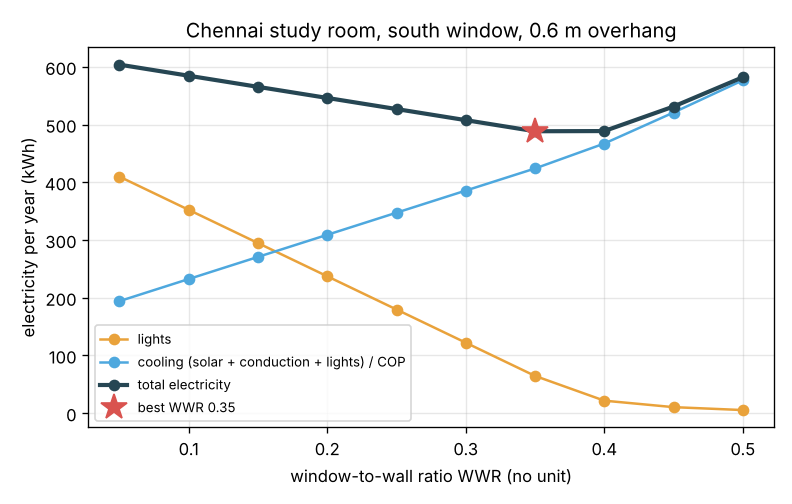
\includegraphics[width=0.85\linewidth]{figures/s03_energy_vs_wwr.png}\\\small Yearly electricity for lights, cooling and total against the window-to-wall ratio (Chennai, south, 0.6 m overhang).\end{center}

\begin{center}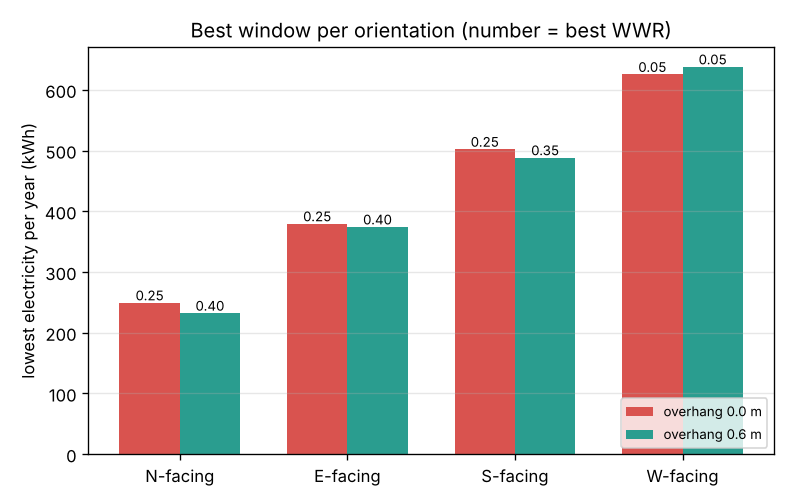
\includegraphics[width=0.85\linewidth]{figures/s03_best_by_orientation.png}\\\small Lowest yearly electricity and the best WWR for each orientation, with and without a 0.6 m overhang.\end{center}

\subsection*{E. Worked example}
The Chennai study room (4 m facade, 5 m deep, 3 m high) has a south window with WWR 0.25 (2 m x 1.5 m = 3 m2) and a 0.6 m overhang 0.3 m above it. Find the visible sky angle, the average daylight factor and the yearly electricity, and check the totals by hand.
\begin{enumerate}[nosep]
\item Visible sky angle: theta = atan((0.3 + 0.75) / 0.6) = atan(1.75) = 60.26 degrees.
\item Room surface area: 2 x (4 x 5 + 4 x 3 + 5 x 3) = 94 m2. DF = 0.7 x 3 x 60.26 / (94 x (1 - 0.25)) = 126.5 / 70.5 = 1.79 percent (below the 2 percent target).
\item The year simulation (365 days x 96 quarter hours) gives: solar heat during use 729.1 kWh, lights 179.5 kWh (out of a maximum of 8 W/m2 x 20 m2 x 8 h x 365 = 467 kWh).
\item Conduction by hand: (5.8 - 2.0) x 3 m2 x 4 K x 8 h x 365 days / 1000 = 133.2 kWh.
\item Cooling electricity = (729.1 + 133.2 + 179.5) / 3 = 347.2 kWh. Total = 179.5 + 347.2 = 526.8 kWh per year.
\item Checks: the 3D ray test and the VSA formula agree within 0.0002; halving the time step changes the total by less than 0.01 kWh.
\end{enumerate}
\textbf{Answer.} theta = 60.26 degrees, DF = 1.79 percent, total about 527 kWh per year (lights 180, cooling 347).

\subsection*{F. Questions}
\begin{enumerate}[nosep]
\item \textbf{Conceptual.} Why is there a best window size, rather than "the bigger the better" or "the smaller the better"?
\item \textbf{Numerical.} For the north window of the mini-project (WWR 0.35, 0.3 m overhang 0.3 m above a 1.5 m window), find the glass area, the visible sky angle and the average daylight factor. Does it meet 2 percent?
\item \textbf{Graph and simulation interpretation.} In Figure 1, by how much do lighting and cooling change from WWR 0.30 to 0.35, and from 0.40 to 0.45? Use this to explain where the minimum lies.
\item \textbf{Design and optimisation challenge.} Design: your client insists on a west-facing window (the view is to the west) and needs DF of at least 2 percent. Using the model, what is the best you can do with the overhang options 0 to 0.9 m? Suggest two design changes outside the model that would help, and say how you would test them.
\end{enumerate}

\section{Real-world mini-project}
\textbf{Plan the window of a study room in Chennai.} A student's study room in Chennai (13 N) is 4 m wide, 5 m deep and 3 m high, used from 9:00 to 17:00 with a 300 lux task light that dims when daylight is available, and an air conditioner with COP 3. The single outside wall can face north, east, south or west (the plot allows any). Window heights are 1.5 m with a 0.3 m gap to the overhang; the overhang can be 0, 0.3, 0.6 or 0.9 m deep; the WWR can be 0.05 to 0.5 in steps of 0.05. The room must have an average daylight factor of at least 2 percent. Use \texttt{simulate\_year} and \texttt{plan\_window} from Session 3.

\section{The path ahead}
\begin{enumerate}[nosep]
\item \textbf{Session 4: Clock time, the equation of time and real sunrise.} A function that converts IST at a given longitude to solar time, and a sunrise and sunset in clock time with the standard 0.833 degree correction.
\item \textbf{Session 5: Side fins and egg-crate shading.} A fin shading function for one or two fins and a combined overhang-plus-fin (egg-crate) sunlit area, checked with the 3D ray test of Session 3.
\item \textbf{Session 6: Real weather and the monsoon.} A reader for an hourly weather file and a version of \texttt{simulate\_year} that uses measured direct and diffuse sunlight and the outdoor temperature instead of the clear-sky model and a fixed 4 K.
\item \textbf{Session 7: A daylight map across the room.} A grid of desk points with a sky component from the visible sky patch and a simple internally reflected component, and the share of working hours each point gets 300 lux.
\item \textbf{Session 8: Glare and thermal mass.} A check for sun patches on a desk zone, and a one-node resistance-capacitance (RC) room model that stores heat between hours.
\end{enumerate}

\section{Answers and hints}

\subsection*{Session 1}
\begin{enumerate}[nosep]
\item \textbf{Conceptual.} Hint: Compare the latitude with the range of the declination, -23.45 to +23.45 degrees. Solution: The noon altitude is 90 - |phi - delta|. In Delhi phi = 28.6, so phi - delta goes from 5.15 (June) to 52.05 (December): the noon sun is high in June and low in December. The noon sun is north of the zenith only when delta > phi. The declination never exceeds 23.45, so this happens only for latitudes below 23.45 N. Chennai (13 N) qualifies from late April to mid August; Delhi (28.6 N) never does.
\item \textbf{Numerical.} Hint: Noon altitude = 90 - |13 - 23.45|; is phi bigger or smaller than delta? Solution: Altitude = 90 - 10.45 = 79.55 degrees. Shadow = 1 / tan(79.55) = 0.184 m. Because delta > phi the sun is to the north, so the shadow points south. Day length: cos H0 = -tan(13) tan(23.45) = -0.231 x 0.434 = -0.100, H0 = 95.7 degrees, day = 12.77 h. Sanity check: just over 12 h, as expected near the equator in summer.
\item \textbf{Graph and simulation interpretation.} Hint: A zero crossing means the noon sun is exactly overhead: delta = phi. Solution: Chennai crosses twice: about day 115 (25 April) and day 229 (17 August), when the declination passes through 13 degrees on its way up and down. Delhi needs delta = 28.6, which never happens, so its curve stays positive (shadow always to the north). It is longest at the winter solstice, 21 December, when the sun is lowest (37.95 degrees, shadow 1.28 m for a 1 m pole).
\item \textbf{Design and optimisation challenge.} Hint: The wall's noon shadow length is 2.4 / tan(alpha); compare it with the 3 m gap. Solution: On 21 December alpha = 37.95 degrees, so the wall's shadow is 2.4 / 0.780 = 3.08 m: it just reaches past the 3 m gap and shades the foot of the window. A gap of at least 3.08 m (say 3.1 m) keeps the whole window in noon sun. On 21 June alpha = 84.85 degrees and the shadow is only 0.22 m, so the courtyard is almost fully sunlit. Trade-off: a wider courtyard gives winter sun but more summer sun on the ground; trees or a pergola can shade it in summer.
\end{enumerate}

\subsection*{Session 2}
\begin{enumerate}[nosep]
\item \textbf{Conceptual.} Hint: Compare the vertical shadow angle of the high midday sun on a south wall with that of the low afternoon sun on a west wall. Solution: On a south wall the summer sun at midday is high and nearly in front, so the VSA is large (85 degrees at June noon): even a short overhang throws a long shadow down the wall. A west window receives the sun in the late afternoon, when it is low and nearly in front of the wall, so the VSA is small (for example 20 to 35 degrees): the overhang would need to be deeper than the window is tall. West windows need vertical fins, screens (jaalis), trees or simply a smaller size.
\item \textbf{Numerical.} Hint: gamma = 289.71 - 270; tan(VSA) = tan(32.44) / cos(gamma). Solution: gamma = 19.71 degrees. cos(theta) = cos(32.44) x cos(19.71) = 0.844 x 0.941 = 0.794. tan(VSA) = 0.636 / 0.941 = 0.675, VSA = 34.0 degrees. Shadow reach = 0.5 x 0.675 = 0.338 m; minus the 0.3 m gap leaves 0.038 m shaded, so 97.5 percent of the window is in sun. Sanity check: the overhang almost does nothing against the low western sun.
\item \textbf{Graph and simulation interpretation.} Hint: Where does the sun rise and set in June at 28.6 N (Session 1)? Solution: December: the south window (8.7 kWh per day), because the low winter sun is in front of it all day. June: east and west (6.2 kWh each), because the summer sun rises and sets well north of east and west and shines on them at a low angle for hours, while the high noon sun hits the south wall at a glancing angle (1.4 kWh). The north window gets 2.6 kWh in June: early morning and late afternoon sun from the north-east and north-west, plus diffuse light.
\item \textbf{Design and optimisation challenge.} Hint: P = (G + H) / tan(VSA), and for a south wall at noon VSA = altitude. Solution: P = (0.3 + 1.5) / tan(61.4) = 1.8 / 1.834 = 0.98 m. On 21 December: reach = 0.98 x 0.780 = 0.765 m, minus 0.3 gives 0.465 m shaded, so 1 - 0.465 / 1.5 = 0.69 (69 percent) sunlit. A 1 m overhang would leave 68 percent sunlit. Trade-off: a deeper overhang extends the shaded season into early autumn but cuts winter sun; because the sun path is symmetric about the solstice, the overhang treats March (often pleasant) the same as September (often still hot), a seasonal mismatch that adjustable shades or deciduous plants solve.
\end{enumerate}

\subsection*{Session 3}
\begin{enumerate}[nosep]
\item \textbf{Conceptual.} Hint: Look at how the lighting and cooling curves change with WWR in Figure 1, and where each one stops changing. Solution: Lighting energy falls as the window grows, but only until the daylight reaches 300 lux for most working hours; after that (WWR about 0.4 here) extra glass saves almost nothing. Cooling energy keeps rising roughly in proportion to the glass area, because every extra square metre lets in more solar heat and conduction. The sum of a falling curve that flattens out and a rising line has a minimum in between. The position of the minimum depends on the climate, the orientation, the shading, the glass and the lights.
\item \textbf{Numerical.} Hint: Aw = 0.35 x 12 m2; theta = atan((0.3 + 0.75) / 0.3). Solution: Aw = 4.2 m2 (2.8 m x 1.5 m). theta = atan(1.05 / 0.3) = atan(3.5) = 74.05 degrees. DF = 0.7 x 4.2 x 74.05 / (94 x 0.75) = 217.7 / 70.5 = 3.09 percent. Yes, it meets the 2 percent target comfortably. Sanity check: removing the overhang (theta = 90) would give 3.75 percent.
\item \textbf{Graph and simulation interpretation.} Hint: Read the values: lights 122.0, 64.5, 21.6, 10.4; cooling 385.5, 423.9, 467.0, 520.8 kWh. Solution: From 0.30 to 0.35 lights fall by 57.5 kWh and cooling rises by 38.4 kWh: the total falls by 19.1 kWh, so a bigger window still pays. From 0.40 to 0.45 lights fall by only 11.2 kWh but cooling rises by 53.8 kWh: the total rises by 42.6 kWh. The minimum lies where the two changes balance, between 0.35 and 0.40 (488.3 and 488.6 kWh, practically equal).
\item \textbf{Design and optimisation challenge.} Hint: Run \texttt{plan\_window(13.0, facings=(270,))} and look at what an overhang does to the late-afternoon sun (Session 2, question B). Solution: The best is an unshaded west window with WWR 0.2 (DF 2.14 percent) at about 633 kWh per year, nearly three times the north window. Overhangs reduce the daylight factor more than they cut the low western sun, so they do not help. Better options: vertical fins or a jaali screen that block sun from low westerly angles while keeping part of the view; low-SHGC (solar control) glass, for example 0.3 instead of 0.6; or a tree or a verandah to the west. Test them by adding a fin shading function or changing \texttt{shgc} in \texttt{simulate\_year} and comparing the yearly total, keeping DF at 2 percent or more.
\end{enumerate}

\section{How to join}
Read \texttt{CONTRIBUTING.md} in the repository, then pick an issue labelled \texttt{good first issue}. Repository: \url{https://github.com/KrunalPanchal1995/pan-iit-oss/tree/main/opendaylight}

\end{document}
